\documentclass[t,8pt]{beamer}
%\usetheme{boxes}
%\usecolortheme{default}

%%% packages
\geometry{paperwidth=140mm,paperheight=105mm}
\usefonttheme[onlymath]{serif}

\usepackage{kotex,amsmath,tabto,setspace,tikz}

\usepackage{xcolor}

%%% counters, commands, environments
\newcounter{num}
\resetcounteronoverlays{num}

\newenvironment{defi}[1]{\refstepcounter{num}\begin{block}{정의 \arabic{num}#1}}{\end{block}}
\newenvironment{theo}[1]{\refstepcounter{num}\begin{block}{정리 \arabic{num}#1}}{\end{block}}
\newenvironment{prob}[1]{\refstepcounter{num}\begin{block}{문제 \arabic{num}#1}}{\end{block}}
\newenvironment{exam}[1]{\refstepcounter{num}\begin{block}{예시 \arabic{num}#1}}{\end{block}}

\newcommand{\pb}[1]%\Phantom + fBox
{\fbox{\phantom{\ensuremath{#1}}}}
\newcommand{\rb}[2]%\Red+fBox
{\fbox{\uncover<#1>{\red{\ensuremath{#2}}}}}
\newcommand{\re}[2]%\Red+equation
{\uncover<#1>{\red{\ensuremath{#2}}}}
\renewcommand{\arraystretch}{1.5}
\newcommand{\red}[1]{\color{red}{#1}}
\newcommand{\ivs}{\centering\strut\vspace*{-\baselineskip}\newline}%image vertical setting
\newcommand*\circled[1]{\tikz[baseline=(char.base)]{\node[shape=circle,draw,inner sep=2pt] (char) {#1};}}

\newcommand{\ar}[1]{\ensuremath{\text{평균변화율}[#1]}}
\newcommand{\ir}[1]{\ensuremath{\text{미분계수}[#1]}}

%%% title
\title{수학 II : 02 미분법}
\institute[ibedu]{아이비에듀}
\date{\today}

%%% toc
\AtBeginSection[]
{\begin{frame}
    \frametitle{목차}
    \tableofcontents[currentsection]
  \end{frame}}


\begin{document}
%%
\frame{\titlepage}

%%%%
\section{미분계수와 도함수}

%%%
\subsection{평균변화율}

%%
\begin{frame}[t]{\subsecname}
\begin{minipage}{.6\textwidth}
%
\begin{defi}{) 평균변화율}\:\par
함수 \(y=f(x)\)의 \([a,b]\)에서의 평균변화율은
\[\ar{f(x),a,b}=\frac{f(b)-f(a)}{b-a}\]
이다.
이 값은 \(x\)의 변화량에 따른 \(f(x)\)의 변화량의 비율을 의미한다.
\(x\)의 변화량은 \(\Delta x\)라고 표시하고, \(f(x)\)의 변화량은 \(\Delta y\)라고 표시한다.
\[\Delta x= b-a,\quad \Delta y=f(b)-f(a).\]
따라서
\[\frac{f(b)-f(a)}{b-a}=\frac{\Delta y}{\Delta x}=\frac{f(a+\Delta x)-f(a)}{\Delta x}\]
이다.
이때, \alert{평균변화율}은, 두 점 \(A(a,f(a))\), \(B(b,f(b))\)을 잇는 직선의 기울기와 같다.
\end{defi}
\end{minipage}
\begin{minipage}{.35\textwidth}
\centering
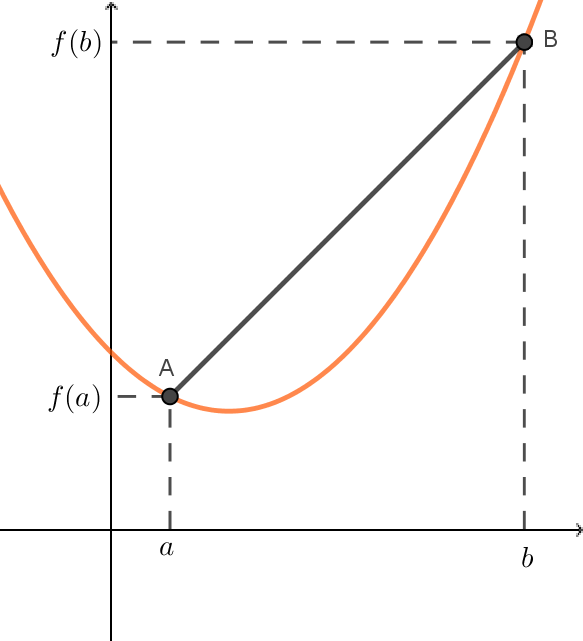
\includegraphics[width=.8\textwidth]{img/1-1-1}
\end{minipage}
\end{frame}

%%
\begin{frame}[t]{\subsecname}
%
\begin{prob}{) 평균변화율을 계산하여라.}\:\par
\begin{minipage}[t]{.48\textwidth}
\centering
(1) \(f(x)=x^2\),\quad \(a=1\), \(b=2\)\\[10pt]
\includegraphics<1>[width=.8\textwidth]{img/1-2-55}
\includegraphics<2>[width=.8\textwidth]{img/1-2-1}
\begin{gather*}
A=\left(\rb21,\rb21\right),\quad B=\left(\rb22,\rb24\right)\\
\Delta x=\rb21,\quad
\Delta y=\rb23\\
\ar{x^2,0,2}=\rb23
\end{gather*}
\end{minipage}
\begin{minipage}[t]{.48\textwidth}
\centering
(2) \(f(x)=2x-4\),\quad \(a=1\), \(b=4\)\\[10pt]
\includegraphics<1>[width=.8\textwidth]{img/1-2-55}
\includegraphics<2>[width=.8\textwidth]{img/1-2-2}
\begin{gather*}
A=\left(\rb21,\rb2{-2}\right),\quad B=\left(\rb24,\rb24\right)\\
\Delta x=\rb23,\quad\Delta y=\rb26\\
\ar{x^2,0,2}=\rb22
\end{gather*}
\end{minipage}
\end{prob}
\end{frame}

%%
\begin{frame}[t]{\subsecname}
%
\begin{prob}{) 평균변화율을 계산하여라.}\:\par
\begin{minipage}[t]{.48\textwidth}
\centering
(3) \(f(x)=-x^2+2\),\quad \(a=-1\), \(b=2\)\\[10pt]
\includegraphics<1>[width=.8\textwidth]{img/1-2-55}
\includegraphics<2>[width=.8\textwidth]{img/1-2-3}
\begin{gather*}
A=\left(\rb2{-1},\rb21\right),\quad B=\left(\rb22,\rb2{-2}\right)\\
\Delta x=\rb23,\quad \Delta y=\rb2{-3}\\
\ar{x^2,0,2}=\rb2{-1}
\end{gather*}
\end{minipage}
\begin{minipage}[t]{.48\textwidth}
\centering
(4) \(f(x)=3\),\quad \(a=3\), \(b=4\)\\[10pt]
\includegraphics<1>[width=.8\textwidth]{img/1-2-55}
\includegraphics<2>[width=.8\textwidth]{img/1-2-4}
\begin{gather*}
A=\left(\rb23,\rb23\right),\quad B=\left(\rb24,\rb23\right)\\
\Delta x=\rb21,\quad \Delta y=\rb20\\
\ar{x^2,0,2}=\rb20
\end{gather*}
\end{minipage}
\end{prob}
\end{frame}

%%%
\subsection{미분계수(순간변화율)}

%%
\begin{frame}[t]{\subsecname}
\begin{minipage}{.6\textwidth}
%
\begin{defi}{) 순간변화율}\:\par
함수 \(f(x)\)의 \(x=a\)에서의 \alert{미분계수}는 (또는 \alert{순간변화율}은)
\[f'(a)=\lim_{x\to a}\frac{f(x)-f(a)}{x-a}\]
이다.
%미분계수 \(f'(a)\)가 존재하면 \(f(x)\)는 \(x=a\)에서 \alert{미분 가능}하다고 말한다.
\(\Delta x = x-a\)라고 두면 위의 식은
\[f'(a)=\lim_{\Delta x\to 0}\frac{f(a+\Delta x)-f(a)}{\Delta x}\]
가 된다.
미분계수 \(f'(a)\)는 점 \(A(a,f(a))\)에서의 접선의 기울기와 같다.
\end{defi}
\end{minipage}
\begin{minipage}{.35\textwidth}
\centering
\includegraphics<1>[width=.8\textwidth]{img/1-3-1}
\includegraphics<2>[width=.8\textwidth]{img/1-3-2}
\end{minipage}
\end{frame}

%%
\begin{frame}[t]{\subsecname}
%
\begin{prob}{) 순간변화율을 계산하여라.}\:\par
\begin{minipage}[t]{.48\textwidth}
\centering
(1) \(f(x)=x^2\),\quad \(a=1\)\\[10pt]
\includegraphics<1>[width=.8\textwidth]{img/1-1-55}
\includegraphics<2>[width=.8\textwidth]{img/1-2-5}
\begin{gather*}
f'(1)=\rb22
\end{gather*}
\end{minipage}
\begin{minipage}[t]{.48\textwidth}
\centering
(2) \(f(x)=2x-4\),\quad \(a=1\)\\[10pt]
\includegraphics<1>[width=.8\textwidth]{img/1-1-55}
\includegraphics<2>[width=.8\textwidth]{img/1-2-6}
\begin{gather*}
f'(1)=\rb22
\end{gather*}
\end{minipage}
\end{prob}
\end{frame}

%%
\begin{frame}[t]{\subsecname}
%
\begin{prob}{) 순간변화율을 계산하여라.}\:\par
\begin{minipage}[t]{.48\textwidth}
\centering
(3) \(f(x)=-x^2+2\),\quad \(a=-1\)\\[10pt]
\includegraphics<1>[width=.8\textwidth]{img/1-1-55}
\includegraphics<2>[width=.8\textwidth]{img/1-2-7}
\begin{gather*}
f'(-1)=\rb22
\end{gather*}
\end{minipage}
\begin{minipage}[t]{.48\textwidth}
\centering
(4) \(f(x)=3\),\quad \(a=3\)\\[10pt]
\includegraphics<1>[width=.8\textwidth]{img/1-1-55}
\includegraphics<2>[width=.8\textwidth]{img/1-2-8}
\begin{gather*}
f'(3)=\rb20
\end{gather*}
\end{minipage}
\end{prob}
\end{frame}

%%%
\subsection{미분가능성과 연속성}

%%
\begin{frame}[t]{\subsecname}
%
\begin{defi}{) 미분가능성}\:\par
함수 \(f(x)\)에 대하여 미분계수 \(f'(a)\)가 존재하면 \(f(x)\)는 \(x=a\)에서 \alert{미분가능}하다고 말한다.
\end{defi}
\begin{align*}
\text{\(f(x)\)는 \(x=a\)에서 \alert{미분가능}하다}
\iff&\text{\(f'(a)\)가 존재한다.}\\
\iff&\text{\(\lim_{x\to a}\frac{f(x)-f(a)}{x-a}\)가 존재한다.}\\
\iff&\lim_{x\to a-}\frac{f(x)-f(a)}{x-a}=\lim_{x\to a+}\frac{f(x)-f(a)}{x-a}\\[10pt]
\iff&\text{좌미분계수} = \text{우미분계수}
\end{align*}

\end{frame}

%%
\begin{frame}[t]{\subsecname}
%
\begin{prob}{) 다음 함수의 미분가능성을 조사하여라.}\:\par
\begin{minipage}[t]{.48\textwidth}
\centering
(1) \(f(x)=x^2\)\\[10pt]
\includegraphics<1>[width=.8\textwidth]{img/1-4-55}
\includegraphics<2>[width=.8\textwidth]{img/1-4-1}
\\[10pt]\scalebox{.9}{\(\lim_{x\to1-}\limits\frac{f(x)-f(1)}{x-1}=\rb22\:\lim_{x\to1+}\limits\frac{f(x)-f(1)}{x-1}=\rb22\)}\par\medskip
\small
\(f(x)\)는 \(x=1\)에서 ({\color<2>{red}{미분가능}}/미분불가능)하다.\par\medskip
\(f(x)\)는 \(x=2\)에서 ({\color<2>{red}{미분가능}}/미분불가능)하다.\par\medskip
\(f(x)\)는 \(\rb2{(-\infty,\infty)}\)에서 미분가능하다.\par\medskip
\end{minipage}
\begin{minipage}[t]{.48\textwidth}
\centering
(2) \(f(x)=\begin{cases}-x^2+1&(x\le 1)\\-x^2+4x-3&(x>1)\end{cases}\)\\[10pt]
\includegraphics<1>[width=.8\textwidth]{img/1-4-55}
\includegraphics<2>[width=.8\textwidth]{img/1-4-2}
\\[10pt]\scalebox{.9}{\(\lim_{x\to1-}\limits\frac{f(x)-f(1)}{x-1}=\rb2{-2}\:\lim_{x\to1+}\limits\frac{f(x)-f(1)}{x-1}=\rb22\)}\par\medskip
\small
\(f(x)\)는 \(x=1\)에서 (미분가능/{\color<2>{red}{미분불가능}})하다.\par\medskip
\(f(x)\)는 \(x=2\)에서 ({\color<2>{red}{미분가능}}/미분불가능)하다.\par\medskip
\(f(x)\)는 \(\rb2{(-\infty,1)}\), \(\rb2{(1,\infty)}\)에서 미분가능하다.\par\medskip
\end{minipage}
\end{prob}
\end{frame}

%%
\begin{frame}[t]{\subsecname}
%
\begin{prob}{) 다음 함수의 미분가능성을 조사하여라.}\:\par
\begin{minipage}[t]{.48\textwidth}
\centering
(3) \(f(x)=\begin{cases}x+2&(x\le-1)\\x^2&(x>-1)\end{cases}\)\\[10pt]
\includegraphics<1>[width=.8\textwidth]{img/1-4-55}
\includegraphics<2>[width=.8\textwidth]{img/1-4-3}
\\[10pt]\scalebox{.9}{\(\lim_{x\to-1-}\limits\frac{f(x)-f(-1)}{x+1}=\rb21\:\lim_{x\to-1+}\limits\frac{f(x)-f(-1)}{x+1}=\rb2{-2}\)}\par\medskip
\small
\(f(x)\)는 \(x=-1\)에서 ({\color<2>{red}{미분가능}}/미분불가능)하다.\par\medskip
\(f(x)\)는 \(x=1\)에서 (미분가능/{\color<2>{red}{미분불가능}})하다.\par\medskip
\(f(x)\)는 \(\rb2{(-\infty,-1)}\), \(\rb2{(-1,\infty)}\)에서 미분가능하다.\par\medskip
\end{minipage}
\begin{minipage}[t]{.48\textwidth}
\centering
(4) \(f(x)=|x|\)\\[10pt]
\includegraphics<1>[width=.8\textwidth]{img/1-4-55}
\includegraphics<2>[width=.8\textwidth]{img/1-4-4}
\\[10pt]\scalebox{.9}{\(\lim_{x\to0-}\limits\frac{f(x)-f(0)}{x-0}=\rb2{-1}\:\lim_{x\to0+}\limits\frac{f(x)-f(0)}{x-0}=\rb21\)}\par\medskip
\small
\(f(x)\)는 \(x=0\)에서 (미분가능/{\color<2>{red}{미분불가능}})하다.\par\medskip
\(f(x)\)는 \(x=1\)에서 ({\color<2>{red}{미분가능}}/미분불가능)하다.\par\medskip
\(f(x)\)는 \(\rb2{(-\infty,0)}\), \(\rb2{(0,\infty)}\)에서 미분가능하다.\par\medskip
\end{minipage}
\end{prob}
\end{frame}

%%
\begin{frame}[t]{\subsecname}
%
\begin{prob}{) 다음 함수의 미분가능성을 조사하여라.}\:\par
\begin{minipage}[t]{.48\textwidth}
\centering
(5) \(f(x)=x-3+|x-2|\)\\[10pt]
\includegraphics<1>[width=.8\textwidth]{img/1-4-55}
\includegraphics<2>[width=.8\textwidth]{img/1-4-5}
\\[10pt]\scalebox{.9}{\(\lim_{x\to2-}\limits\frac{f(x)-f(2)}{x-2}=\rb20\:\lim_{x\to2+}\limits\frac{f(x)-f(2)}{x-2}=\rb22\)}\par\medskip
\small
\(f(x)\)는 \(x=1\)에서 ({\color<2>{red}{미분가능}}/미분불가능)하다.\par\medskip
\(f(x)\)는 \(x=2\)에서 (미분가능/{\color<2>{red}{미분불가능}})하다.\par\medskip
\(f(x)\)는 \(\rb2{(-\infty,2)}\), \(\rb2{(2,\infty)}\)에서 미분가능하다.\par\medskip
\end{minipage}
\begin{minipage}[t]{.48\textwidth}
\centering
(6) \(f(x)=\begin{cases}-x^2&(x<0)\\x^2&(x\ge0)\end{cases}\)\\[10pt]
\includegraphics<1>[width=.8\textwidth]{img/1-4-55}
\includegraphics<2>[width=.8\textwidth]{img/1-4-6}
\\[10pt]\scalebox{.9}{\(\lim_{x\to0-}\limits\frac{f(x)-f(0)}{x-0}=\rb20\:\lim_{x\to0+}\limits\frac{f(x)-f(0)}{x-0}=\rb20\)}\par\medskip
\small
\(f(x)\)는 \(x=0\)에서 ({\color<2>{red}{미분가능}}/미분불가능)하다.\par\medskip
\(f(x)\)는 \(x=1\)에서 ({\color<2>{red}{미분가능}}/미분불가능)하다.\par\medskip
\(f(x)\)는 \(\rb2{(-\infty,\infty)}\)에서 미분가능하다.\par\medskip
\end{minipage}
\end{prob}
\end{frame}

%%
\begin{frame}[t]{\subsecname}
%
\begin{prob}{) 다음 함수의 미분가능성을 조사하여라.}\:\par
\begin{minipage}[t]{.48\textwidth}
\centering
(7) \(f(x)=\begin{cases}-x^2&(x\le1)\\-x+3&(x>1)\end{cases}\)\\[10pt]
\includegraphics<1>[width=.8\textwidth]{img/1-4-55}
\includegraphics<2>[width=.8\textwidth]{img/1-4-7}
\\[10pt]\scalebox{.9}{\(\lim_{x\to1-}\limits\frac{f(x)-f(1)}{x-1}=\rb22\:\lim_{x\to1+}\limits\frac{f(x)-f(1)}{x-1}=\rb2\times\)}\par\medskip
\small
\(f(x)\)는 \(x=1\)에서 (미분가능/{\color<2>{red}{미분불가능}})하다.\par\medskip
\(f(x)\)는 \(x=2\)에서 ({\color<2>{red}{미분가능}}/미분불가능)하다.\par\medskip
\(f(x)\)는 \(\rb2{(-\infty,1)}\), \(\rb2{(1,\infty)}\)에서 미분가능하다.\par\medskip
\end{minipage}
\begin{minipage}[t]{.48\textwidth}
\centering
(8) \(f(x)=\frac{|x|}x\)\\[10pt]
\includegraphics<1>[width=.8\textwidth]{img/1-4-55}
\includegraphics<2>[width=.8\textwidth]{img/1-4-8}
\\[10pt]\scalebox{.9}{\(\lim_{x\to0-}\limits\frac{f(x)-f(0)}{x-0}=\rb2\times\:\lim_{x\to0+}\limits\frac{f(x)-f(0)}{x-0}=\rb2\times\)}\par\medskip
\small
\(f(x)\)는 \(x=0\)에서 (미분가능/{\color<2>{red}{미분불가능}})하다.\par\medskip
\(f(x)\)는 \(x=1\)에서 ({\color<2>{red}{미분가능}}/미분불가능)하다.\par\medskip
\(f(x)\)는 \(\rb2{(-\infty,0)}\), \(\rb2{(0,\infty)}\)에서 미분가능하다.\par\medskip
\end{minipage}
\end{prob}
\end{frame}



%%%
\subsection{도함수}
%%
\begin{frame}[t]{\subsecname}
\begin{minipage}[t]{.48\textwidth}
%
\begin{prob}{) \(f(x)=x^2\)}
\vspace{-10pt}
\begin{align*}
f'(1)
&=\uncover<2>{\lim_{h\to0}\frac{f(1+h)-f(1)}h\\
&=\lim_{h\to0}\frac{(1+h)^2-1}h\\
&=\lim_{h\to0}(h+2)\\
&=\red2}\\
f'(2)
&=\uncover<2>{\lim_{h\to0}\frac{f(2+h)-f(2)}h\\
&=\lim_{h\to0}\frac{(2+h)^2-4}h\\
&=\lim_{h\to0}(h+4)\\
&=\red4}\\
f'(x)
&=\uncover<2>{\lim_{h\to0}\frac{f(x+h)-f(x)}h\\
&=\lim_{h\to0}\frac{(x+h)^2-x^2}h\\
&=\lim_{h\to0}(h+2x)\\
&=\red{2x}}
\end{align*}
\end{prob}
\end{minipage}
\begin{minipage}[t]{.48\textwidth}
%
\begin{prob}{) \(f(x)=x^3\)}
\vspace{-10pt}
\begin{align*}
f'(1)
&=\uncover<2>{\lim_{h\to0}\frac{f(1+h)-f(1)}h\\
&=\lim_{h\to0}\frac{(1+h)^3-1}h\\
&=\lim_{h\to0}(h^2+3h+3)\\
&=\red3}\\
f'(2)
&=\uncover<2>{\lim_{h\to0}\frac{f(2+h)-f(2)}h\\
&=\lim_{h\to0}\frac{(2+h)^3-4}h\\
&=\lim_{h\to0}(h^2+6h+12)\\
&=\red{12}}\\
f'(x)
&=\uncover<2>{\lim_{h\to0}\frac{f(x+h)-f(x)}h\\
&=\lim_{h\to0}\frac{(x+h)^3-x^2}h\\
&=\lim_{h\to0}(h^2+3xh+3x^2)\\
&=\red{3x^2}}
\end{align*}
\end{prob}
\end{minipage}
\end{frame}

%%
\begin{frame}[t]{\subsecname}
\begin{minipage}[t]{.48\textwidth}
%
\begin{prob}{) \(f(x)=x\)}
\vspace{-10pt}
\begin{align*}
f'(1)
&=\uncover<2>{\lim_{h\to0}\frac{f(1+h)-f(1)}h\\
&=\lim_{h\to0}\frac{(1+h)-1}h\\
&=\lim_{h\to0}1\\
&=\red1}\\
f'(2)
&=\uncover<2>{\lim_{h\to0}\frac{f(2+h)-f(2)}h\\
&=\lim_{h\to0}\frac{(2+h)-2}h\\
&=\lim_{h\to0}1\\
&=\red1}\\
f'(x)
&=\uncover<2>{\lim_{h\to0}\frac{f(x+h)-f(x)}h\\
&=\lim_{h\to0}\frac{(x+h)-x}h\\
&=\lim_{h\to0}1\\
&=\red1}
\end{align*}
\end{prob}
\end{minipage}
\begin{minipage}[t]{.48\textwidth}
%
\begin{prob}{) \(f(x)=1\)}
\vspace{-10pt}
\begin{align*}
f'(1)
&=\uncover<2>{\lim_{h\to0}\frac{f(1+h)-f(1)}h\\
&=\lim_{h\to0}\frac{1-1}h\\
&=\lim_{h\to0}0\\
&=\red0}\\
f'(2)
&=\uncover<2>{\lim_{h\to0}\frac{f(2+h)-f(2)}h\\
&=\lim_{h\to0}\frac{1-1}h\\
&=\lim_{h\to0}0\\
&=\red0}\\
f'(x)
&=\uncover<2>{\lim_{h\to0}\frac{f(x+h)-f(x)}h\\
&=\lim_{h\to0}\frac{1-1}h\\
&=\lim_{h\to0}0\\
&=\red0}
\end{align*}
\end{prob}
\end{minipage}
\end{frame}

%%
\begin{frame}[t]{\subsecname}
%
\begin{theo}{}
자연수 \(n\)에 대하여 \(f(x)=x^n\)이면 \(f'(x)=nx^{n-1}\)이다.
\[\left(x^n\right)'=nx^{n-1}\]
\end{theo}
%
\begin{prob}{) \(f'(x)\)를 구하여라.}
\begin{enumerate}[(1)]
\setlength{\itemsep}{10pt}
\item
\(f(x)=x\)\\[10pt]
\(f'(x) = \re21\)
\item
\(f(x)=x^4\)\\[10pt]
\(f'(x) = \re2{4x^3}\)
\item
\(f(x)=x^7\)\\[10pt]
\(f'(x) = \re2{7x^6}\)
\item
\(f(x)=x^{100}\)\\[10pt]
\(f'(x) = \re2{100x^{99}}\)
\end{enumerate}
\end{prob}
\end{frame}

%%
\begin{frame}[t]{\subsecname}
%
\begin{theo}{}
함수 \(f(x)\), \(g(x)\)가 미분가능하고 \(c\)가 실수일 때,
\begin{enumerate}[(1)]
\setlength{\itemsep}{10pt}
\item
\(\left(cf(x)\right)'=cf'(x)\)
\item
\(\left(f(x)+g(x)\right)'=f'(x)+g'(x)\)
\item
\(\left(f(x)-g(x)\right)'=f'(x)-g'(x)\)
\end{enumerate}
\end{theo}
%
\begin{prob}{) \(f'(x)\)를 구하여라.}
\begin{enumerate}[(1)]
\setlength{\itemsep}{10pt}
\item
\(f(x)=2x^2+3x\)\\[10pt]
\(f'(x) = \re2{4x+3}\)
\item
\(f(x)=x^3-3x^2+2\)\\[10pt]
\(f'(x) = \re2{3x^2-6x}\)
\item
\(f(x)=2x^3-4x^2+3x+1\)\\[10pt]
\(f'(x) = \re2{6x^2-8x+3}\)
\item
\(f(x)=-\frac15x^{10}+\frac12x^3-7\)\\[10pt]
\(f'(x) = \re2{-2x^9+\frac32x^2}\)
\end{enumerate}
\end{prob}
\end{frame}

%%
\begin{frame}[t]{\subsecname}
%
\begin{theo}{) 곱의 미분법}
함수 \(f(x)\), \(g(x)\)가 미분가능할 때,
\[\left(f(x)g(x)\right)'=f'(x)g(x)+f(x)g'(x)\]
\end{theo}
%
\begin{prob}{) \(f'(x)\)를 구하여라.}
\begin{enumerate}[(1)]
\setlength{\itemsep}{10pt}
\item
\(f(x)=(x+2)(x-3)\)\\[10pt]
\(f'(x) = \re2{2x-1}\)
\item
\(f(x)=(x^2+1)(x+3)\)\\[10pt]
\(f'(x) = \re2{3x^2+6x+1}\)
\item
\(f(x)=(x^3+1)(x^2+2)\)\\[10pt]
\(f'(x) = \re2{5x^4+6x^2+2x}\)
\end{enumerate}
\end{prob}
\end{frame}

%%
\begin{frame}[t]{\subsecname}
%
\addtocounter{num}{-2}
\begin{theo}{) 곱의 미분법}
함수 \(f(x)\), \(g(x)\)가 미분가능할 때,
\[\left(f(x)g(x)\right)'=f'(x)g(x)+f(x)g'(x)\]
\end{theo}
\stepcounter{num}
%
\begin{prob}{) 곱의 미분법을 사용하여 다음을 계산하여라.}
\begin{enumerate}[(1)]
\setlength{\itemsep}{20pt}
\setlength{\parsep}{20pt}
\item
\(\left(\left(f(x)\right)^2\right)'=\re2{2f(x)f'(x)}\)
\item
\(\left(f(x)g(x)h(x)\right)'=\re2{f'(x)g(x)h(x)+f(x)g'(x)h(x)+f(x)g(x)h'(x)}\)
\item
\(\left(\left(f(x)\right)^3\right)'=\re2{3\left(f(x)\right)^2f'(x)}\)
\end{enumerate}
\end{prob}
\end{frame}

%%
\begin{frame}[t]{\subsecname}
%
\begin{theo}{}
\(n\)이 자연수이고 함수 \(f(x)\)가 미분가능할 때,
\[\left(\left(f(x)\right)^n\right)'=n\left(f(x)\right)^{n-1}f'(x)\]
\end{theo}
%
\begin{prob}{) \(f'(x)\)를 구하여라.}
\begin{enumerate}[(1)]
\setlength{\itemsep}{10pt}
\item
\(f(x)=(x-2)^2\)\\[10pt]
\(f'(x) = \re2{2x-4}\)
\item
\(f(x)=(x+1)^3\)\\[10pt]
\(f'(x) = \re2{3(x+1)^2}\)
\item
\(f(x)=(2x-1)^4\)\\[10pt]
\(f'(x) = \re2{8(2x-1)^3}\)
\item
\(f(x)=(3x+4)^2\)\\[10pt]
\(f'(x) = \re2{6(3x+4)}\)
\item
\(f(x)=(x^2+x)^5\)\\[10pt]
\(f'(x) = \re2{5(x^2+x)^4(2x+1)}\)
\end{enumerate}
\end{prob}
\end{frame}

%%%%
\section{도함수의 활용}

%%%
\subsection{접선의 방정식}

%%
\begin{frame}[t]{\subsecname}
%
\begin{prob}{) 그래프 \(y=f(x)\) 위의 한 점 \(A\)에서의 접선의 방정식을 구하여라.}\:\par
\begin{minipage}[t]{.48\textwidth}
\centering
(1) \(f(x)=x^2\),\quad \(A=(1,1)\)\\[10pt]
\includegraphics<1>[width=.8\textwidth]{img/1-5-1}
\includegraphics<2>[width=.8\textwidth]{img/1-5-11}
\[y=\re2{2x-1}\]
\end{minipage}
\begin{minipage}[t]{.48\textwidth}
\centering
(2) \(f(x)=x^2\),\quad \(A=(-1,\rb21)\)\\[10pt]
\includegraphics<1>[width=.8\textwidth]{img/1-5-1}
\includegraphics<2>[width=.8\textwidth]{img/1-5-12}
\[y=\re2{-2x-1}\]
\end{minipage}
\end{prob}
\end{frame}

%%
\begin{frame}[t]{\subsecname}
%
\begin{prob}{) 그래프 \(y=f(x)\) 위의 한 점 \(A\)에서의 접선의 방정식을 구하여라.}\:\par
\begin{minipage}[t]{.48\textwidth}
\centering
(3) \(f(x)=-x^2+2x+3\),\quad \(A=(0,\rb23)\)\\[10pt]
\includegraphics<1>[width=.8\textwidth]{img/1-5-2}
\includegraphics<2>[width=.8\textwidth]{img/1-5-21}
\[y=\re2{2x+3}\]
\end{minipage}
\begin{minipage}[t]{.48\textwidth}
\centering
(4) \(f(x)=-x^2+2x+3\),\quad \(A=(1,\rb24)\)\\[10pt]
\includegraphics<1>[width=.8\textwidth]{img/1-5-2}
\includegraphics<2>[width=.8\textwidth]{img/1-5-22}
\[y=\re2{4}\]
\end{minipage}
\end{prob}
\end{frame}

%%
\begin{frame}[t]{\subsecname}
\end{frame}

%%%
\subsection{롤의 정리}

%%
\begin{frame}[t]{\subsecname}
\end{frame}

%%%
\subsection{평균값 정리}

%%
\begin{frame}[t]{\subsecname}
\end{frame}





\end{document}